\documentclass[a4paper,10pt]{article}
\usepackage[utf8]{inputenc}

\usepackage[a4paper]{geometry}
\usepackage{amsmath,amsthm,amssymb,latexsym,amsfonts}
\usepackage{hyperref}
\geometry{hscale=0.75,vscale=0.78,centering}
\usepackage{graphicx}

\usepackage{tikz}

\begin{document}

\begin{titlepage}
    \begin{center}

	\begin{tikzpicture}[remember picture, overlay]
	  \node [anchor=north east, inner sep=0pt]  at (current page.north east)
	     {
\includegraphics[height=3cm]{Banniere_ULB.png}};
	\end{tikzpicture}
	
        {\Large \textbf{\textsc{Faculté des Sciences}}\\
        \textbf{\textsc{Département d'Informatique}}}

        \vfill{}\vfill{}

        \begin{center}
            \Huge{INFO-H-303}
                \Huge{Projet Base de données}
        \end{center}
        \Huge{\par}
        \begin{center}
            \large{
                \textsc{Omer} Nicolas \\
                \textsc{Rosette} Arnaud \\
            }
        \end{center}
        \Huge{\par}

        \vfill{}\vfill{}
        \large{\par}

        \vfill{}\vfill{}\enlargethispage{3cm}

        \begin{figure} [h!]
             \centering
	    
\includegraphics[width=4cm]{Sigle_ULB.png}
	\end{figure}

        \textbf{Année académique 2013~-~2014}
        
    \end{center}
\end{titlepage}

\tableofcontents
\pagebreak

\section{Etude de cas}

Il nous est demandé d'implémenter une application de création de flux d'information RSS 2.0. Il devra être possible pour des utilisateurs de consulter ces flux d'informations (par le biais de publications) et de s'abonner aux flux qui les intéressent. Ce concept est directement inspiré du lecteur de flux \textsl{Google Reader}. De plus, les utilisateurs pourront s'envoyer des demandes d'amitié (afin de s'abonner au flux de leur amis) et partager les publications qui les intéressent. Ils pourront également commenter les publications partagées s'ils le désirent. 

\section{Modèle entité-relation}

Afin de modéliser la façon dont les informations seront physiquement enregistrées en base de données (au moyen d'SQL), voici un diagramme entité-association fournissant une description graphique du modèle conceptuel de données.

\subsection{Schéma}

	\begin{figure}[h!]
	    \centering
	    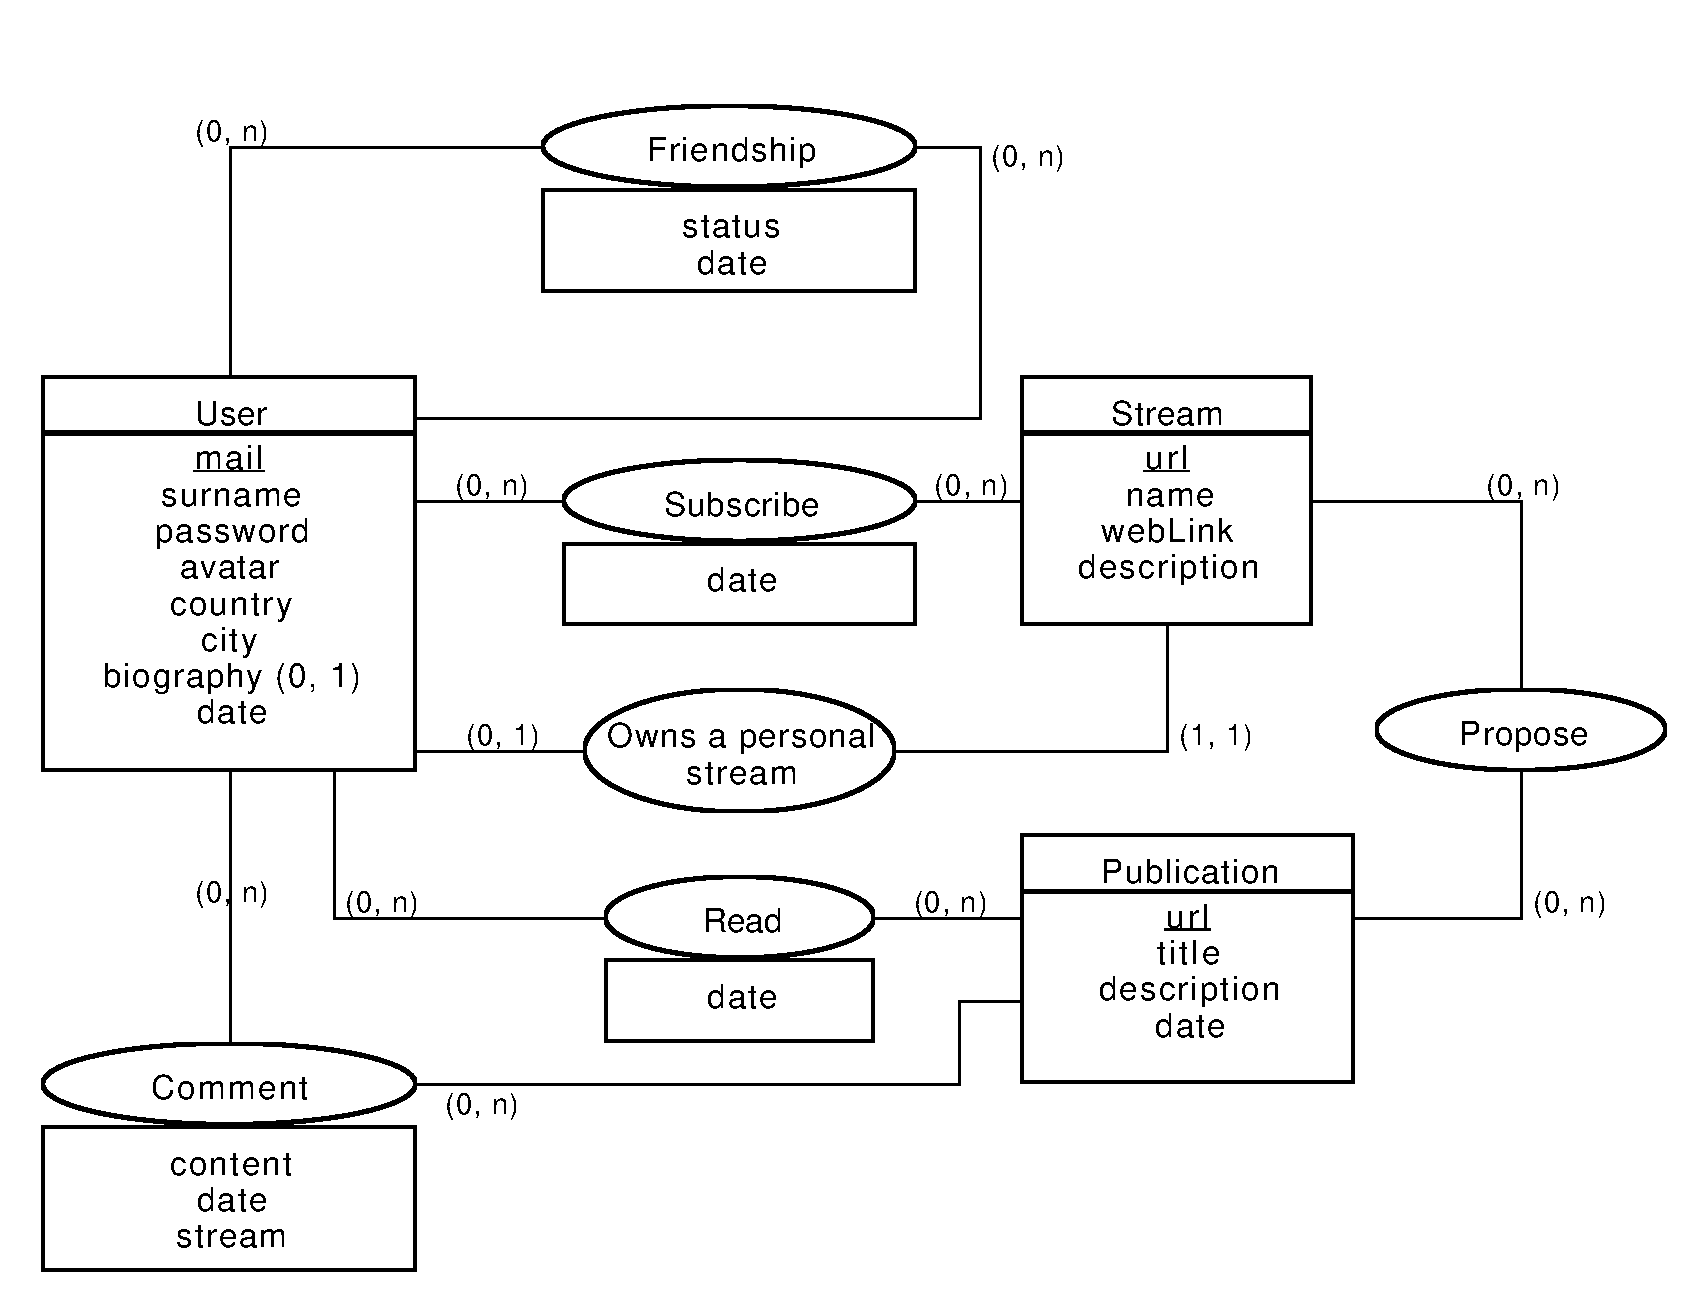
\includegraphics[width=15cm]{Entite-Relation-2.pdf}
	    \caption{Modèle entité-relation de l'application}
	    \label{fig:Entite-Relation}
	\end{figure}

\subsection{Hypothèses du modèle}

La relation \textsl{FriendShip}, une fois traduite en base de données, comprend deux attributs mail\_sender et mail\_receiver (clefs étrangères référençant des champs de la table \textsl{User}). Ces derniers désignent respectivement l'émetteur et le récepteur de la demande d'amitié. On évite ainsi la confusion entre les deux et le cas problématique où l'émetteur de la demande d'amitié aurait accepté le demande sans l'aval du récepteur.

\section{Modèle relationnel}

Cette section comprend quant à elle le modèle logique directement tiré du diagramme entité-association. 

\subsection{Traduction}

User(\underline {mail}, surname, password, avatar, country, city, \textsl{biography},  date, personal\_stream\_url)

personal\_stream\_url référence Stream.url
\\\\
Stream(\underline {url}, name, webLink, description)
\\\\
Publication(\underline {url}, title, date, description)
\\\\
Friendship(\underline {mail\_sender},\underline {mail\_receiver}, status, date)

mail\_sender référence User.mail 

mail\_receiver référence User.mail
\\\\
Comment(\underline {user\_mail}, \underline {publication\_url}, \underline {stream\_url}, content, date)

user\_mail référence User.mail

publication\_url référence Publication.url
\\\\
Read(\underline {user\_mail}, \underline {publication\_url}, date)

user\_mail référence User.mail

publication\_url référence Publication.url
\\\\
Propose(\underline {stream\_url}, \underline {publication\_url})

stream\_url référence Stream.url

publication\_url référence Publication.url
\\\\
Subscribe(\underline {user\_mail}, \underline {stream\_url}, date)

user\_mail référence User.mail

stream\_url référence Stream.url
\\\\

\subsection{Contraintes d’intégrité}

	\begin{itemize}
	    \item Un utilisateur ne peut commenter qu'une seule fois une publication.
	    \item Un utilisateur peut commenter uniquement les publications de son flux personnel ou du flux d'un ami.
	    \item Un utilisateur n'est pas inscrit à son propre flux.
	    \item Un utilisateur ne peut pas envoyer une demande d'ami s'il a déjà reçu une demande du même utilisateur.
	    \item Chaque utilisateur est inscrit au flux de ses amis.
	    \item Sur une publication, un utilisateur ne voit que les commentaires de ses amis.
	    \item La valeur de l'attribut \textsl{date} de la table \textsl{User} doit être antérieure aux valeurs respectives des attributs \textsl{date} de la relation \textsl{Subscribe}, \textsl{date} de la relation \textsl{Read}, \textsl{date} de la relation \textsl{Comment} et \textsl{date} de la relation \textsl{Friendship}.
	    \item La valeur de l'attribut \textsl{date} de la table \textsl{Publication} doit être antérieure aux valeurs respectives des attributs \textsl{date} de la relation \textsl{Read} et date de la relation \textsl{Comment}.
	    \item La valeur de l'attribut \textsl{mail} de la table \textsl{User} doit respecter un format valide, c'est à dire une expression du type : [a-zA-Z0-9+. -] + @[a-z0-9-.] + \.[a-z].
	    \item La valeur des attributs \textsl{date} des tables \textsl{User}, \textsl{Publication}, \textsl{Friendship}, \textsl{Comment}, \textsl{Read} et \textsl{Subscribe} doivent respecter le format suivant : 'yyyy-mm-dd'.
	    \item Un utilisateur ne peut pas s'ajouter lui-même en ami. Il est également impossible d'envoyer une demande à un utilisateur pour lequel il a déjà reçu une demande.
	\end{itemize}

\section{Justification des choix de modélisations}

Nous avions pensé à créer une table \textsl{Personnal Stream} qui héritait de la table \textsl{Stream} mais cela compliquait inutilement le modèle. Dans le même ordre d'idées, il était possible d'avoir une table \textsl{Commented Publication} qui aurait hérité de \textsl{Publication} mais la relation \textsl{Comment} suffit amplement pour ce modèle.

\section{Requêtes demandées}

Cette section présente les six requêtes obligatoires écrites respectivement en forme SQL, en algèbre relationnelle et en calcul relationnel tuple. Cependant, seulement les requêtes 5 et 6 ne doivent pas figurer sous ces deux dernières formes.

	\begin{enumerate}
	    \item Tous les utilisateurs qui ont au plus 2 amis
	    \item La liste des flux auxquels a souscrit au moins un utilisateur qui a souscrit à au moins deux flux auxquels X a souscrit
	    \item La liste des flux auxquels X a souscrit, auxquels aucun de ses amis n’a souscrit et duquel il n’a partagé aucune publication
	    \item La liste des utilisateurs qui ont partagé au moins 3 publications que X a partagé
	    \item La liste des flux auquel un utilisateur est inscrit avec le nombre de publications lues, le nombre de publications partagées, le pourcentage de ces dernières par rapport aux premières, cela pour les 30 derniers jours et ordonnée par le nombre de publications partagées.
	    \item La liste des amis d’un utilisateur avec pour chacun le nombre de publications lues par jour et le nombre d’amis, ordonnée par la moyenne des lectures par jour depuis la date d’inscription de cet ami
	\end{enumerate}
	
\subsection{Requêtes SQL}

	\begin{enumerate}
	    \item 
	    \begin{verbatim}
		SELECT u.*
		FROM User u LEFT JOIN (SELECT * FROM Friendship f1 WHERE f1.status = TRUE) AS f2 
		ON f2.mail_sender = u.mail OR f2.mail_receiver = u.mail
		GROUP BY u.mail
		HAVING COUNT(*) < 3;
             \end{verbatim}
	    \item
             \begin{verbatim}
		<user>
		SELECT DISTINCT s3.*
		FROM Subscribe sub3, Stream s3
		WHERE sub3.stream_url = s3.url AND sub3.user_mail IN
		    (SELECT u1.mail
		    FROM User u1, Stream s2, Subscribe sub2
		    WHERE sub2.user_mail != <user>.mail
		    AND sub2.user_mail = u1.mail 
		    AND sub2.stream_url = s2.url 
		    AND sub2.stream_url IN    
		        (SELECT sub1.stream_url 
		            FROM Subscribe sub1 
		            WHERE sub1.user_mail = <user>.mail)
		    GROUP BY sub2.user_mail
		    HAVING COUNT(*) >= 2);
             \end{verbatim}
	    \item 
	    \item 
	    \item 
	    \item 
	\end{enumerate}

\subsection{Algèbre relationnelle}

% Commandes latex pour l'algèbre relationnelle
% \sigma : sélection
% \pi : projection
% \div : division
% \times : multiplication
% \cap : intersection
% \ast : jointure naturelle
% \Join : jointure 
% \sqsupset : LEFT JOIN
% \sqsubset : RIGHT JOIN

	\begin{enumerate}
	    \item
		\begin{equation}
		\underset{2}{F} \leftarrow \sigma \underset{status = True}{} (Friendship) \\
		\end{equation}
		\begin{equation}
		T \leftarrow User \sqsupset \Join \underset{<mail\_sender = mail \vee mail\_receiver = mail>}{} \underset{2}{F} 
		\end{equation}
		\begin{equation}
		Result \leftarrow \pi \underset{*}{}(mail \  \  \  \sigma \underset{COUNT(*) < 3}{}(T))
		\end{equation}
	    \item
		\begin{equation}
		S1 \leftarrow \pi \underset{stream\_url}{} (\sigma \underset{user\_mail = <user>.mail}{}(Subscribe))`
		\end{equation}
		\begin{equation}
		a \leftarrow (\sigma \underset{user\_mail != <user>.mail \wedge user\_mail = mail}{}(User * Subscribe))
		\end{equation}
		\begin{equation}
		b \leftarrow (\sigma \underset{stream\_url = url \wedge stream\_url\  \cap S1}{}(Stream * Subscribe))
		\end{equation}
		\begin{equation}
		U1 \leftarrow \pi \underset{mail}{} (user\_mail \  \  \  \sigma \underset{COUNT(*) >= 2}{}(a \wedge b))
		\end{equation}
		\begin{equation}
		Result \leftarrow \pi \underset{*}{} (\sigma \underset {stream\_url = url \wedge user\_mail \cap U1}{}(Subscribe * Stream))
		\end{equation}
	    \item 
	          \begin{equation}
		Sub1 \leftarrow \pi \underset{stream\_url}{} (\sigma \underset{user\_mail = <user>.mail}{}(Subscribe))
		\end{equation}
		\begin{equation}
		F1 \leftarrow \pi \underset{mail\_sender}{} (\sigma \underset{mail\_receiver = <user>.mail \wedge status = true}{}(Friendship))
		\end{equation}
		\begin{equation}
		F2 \leftarrow \pi \underset{mail\_sender}{} (\sigma \underset{mail\_sender = <user>.mail \wedge status = true}{}(Friendship))
		\end{equation}
		\begin{equation}
		U \leftarrow \pi \underset{mail}{} (\sigma \underset{(mail \cap F1) \vee (mail \cap F2) }{}(User))
		\end{equation}
		\begin{equation}
		Sub2 \leftarrow \pi \underset{stream\_url}{} (\sigma \underset{user\_mail \cap U}{}(Subscribe))
		\end{equation}
		\begin{equation}
		Prop1 \leftarrow \pi \underset{publication\_url}{} (\sigma \underset{url = publication\_url \wedge stream\_url = <user>.personal\_stream\_url}{}(Propose * Publication ))
		\end{equation}
		\begin{equation}
		Prop2 \leftarrow \pi \underset{stream\_url}{} (\sigma \underset{publication\_url \cap Prop1}{}(Propose))
		\end{equation}
		\begin{equation}
		Result \leftarrow \pi \underset{*}{} (\sigma \underset{(url \cap Sub1) \wedge (url \setminus Sub2) \wedge (url \setminus Prop2)}{}(Stream))
		\end{equation}
	    \item
	         \begin{equation}
		PP \leftarrow \pi \underset{*}{} (\sigma \underset{stream\_url = <user>.personal\_stream\_url}{}(Propose))
		\end{equation}
		\begin{equation}
		PU \leftarrow \pi \underset{*}{} (\sigma \underset{(stream\_url = personal\_stream\_url) \wedge (stream\_url != <user>.personal\_stream\_url)}{}(Propose*User))
		\end{equation}
	         \begin{equation}
		Result \leftarrow \pi \underset{*}{} (mail \  \  \  \sigma \underset{COUNT(*) >= 3}{}(PP \cap PU))
		\end{equation}
	\end{enumerate}
	
\subsection{Calcul relationnel tuple}

% Commandes latex pour le calcul tuple
% \forall : pour tout
% \exists : il existe
% \nexists : il n'existe pas
% \cup : union
% \cap : intersection
% \setminus : différence ensembliste
% \wedge : ET
% \vee : OU
% \rightarrow : =>
% \leftarrow : <=

	\begin{enumerate}
	    \item
		\begin{equation}
		[u.* | \ U(u) \ \wedge \forall \underset{\ \ 2}{u} (U(\underset{\ \ 2}{u}) \rightarrow (( \forall f ( F(f) \rightarrow (f.status = False \wedge(f.mail\_sender = \underset{\ \ 2}{u}.mail \vee 
		\end{equation}
		\begin{equation}
		f.mail\_receiver = \underset{\ \ 2}{u}.mail)))) \vee ( \exists \underset{\ \ 2}{f} (F(\underset{\ \ 2}{f}) \rightarrow (\underset{\ \ 2}{f}.status = True \wedge(\underset{\ \ 2}{f}.mail\_sender = \underset{\ \ 2}{u}.mail \vee 
		\end{equation}  
		\begin{equation}
		\underset{\ \ 2}{f}.mail\_receiver = \underset{\ \ 2}{u}.mail)))) \vee ( \exists \underset{\ \ 3}{f} \underset{\ \ 4}{f} (F(\underset{\ \ 3}{f} ) \rightarrow (\underset{\ \ 3}{f}.status = True \wedge (\underset{\ \ 3}{f}.mail\_sender = \underset{\ \ 2}{u}.mail \vee
		\end{equation}  
		\begin{equation}
		\underset{\ \ 3}{f}.mail\_receiver = \underset{\ \ 2}{u}.mail))) \wedge F(\underset{\ \ 4}{f}) \rightarrow (\underset{\ \ 4}{f}.status = True \wedge (\underset{\ \ 4}{f}.mail\_sender = \underset{\ \ 2}{u}.mail \vee
		\end{equation}
		\begin{equation}
		\underset{\ \ 4}{f}.mail\_receiver = \underset{\ \ 2}{u}.mail)) \wedge (\underset{\ \ 3}{f} \ != \underset{\ \ 4}{f}))))]
		\end{equation}
	    \item
	    \item 
	    \item
	\end{enumerate}

\section{Instructions d'exécution du programme}

Concernant les détails techniques, notre programme est codé sous java et utilise MySQL comme base de données. Il nécessite donc de lancer le serveur mysql avant l'utilisation de l'application.

\end{document}
